\documentclass[11pt, oneside,table]{article}   	% use "amsart" instead of "article" for AMSLaTeX format
%\usepackage{geometry}                		% See geometry.pdf to learn the layout options. There are lots.
\usepackage[margin=.9in]{geometry}
\geometry{letterpaper}                   		% ... or a4paper or a5paper or ... 
%\geometry{landscape}                		% Activate for for rotated page geometry
\usepackage[parfill]{parskip}    		% Activate to begin paragraphs with an empty line rather than an indent
\usepackage{graphicx}				% Use pdf, png, jpg, or eps� with pdflatex; use eps in DVI mode
\usepackage{moreverb}						% TeX will automatically convert eps --> pdf in pdflatex		
\usepackage{amssymb}
\usepackage{mathtools}
\usepackage[framed,numbered,]{mcode}
\usepackage{listings}
\usepackage{xcolor}
\usepackage{amsmath}
\usepackage{placeins}
\usepackage{float}
\restylefloat{table}
\lstset { %
    backgroundcolor=\color{black!7}, % set backgroundcolor
    basicstyle=\footnotesize,% basic font setting
}

\newcommand{\bigo}{$\mathcal{O}$}

\title{MATH 6644\\Project 2}
\author{Stephan Boettcher}
%\date{}                                           % Activate to display a given date or no date

\begin{document}
\maketitle
\section*{Fixed-point and Newton's Method for Nonlinear systems}

{\it Consider the discrete Chandrasekhar H-equation:

$$F_i(\vec{x})=x_i -(1-\frac{c}{2N}\sum\limits^N_{j=1}\frac{\mu_ix_j}{\mu_i+\mu_j})^{-1}=0
$$
where $c \in(0,1)$ is a given constant, $\mu_i=\frac{(i-\frac{1}){2}}{N}$ for $1\le i \le N$ and $N$ is the dimension of the unknown vector $\vec{x}$. Write your own code and compute the solution of the equation for $N=200$ and $c=0.9$ by using:
\begin{enumerate}
\item Fixed-point method,
\item Chord method,
\item Newton method,
\item Shamanskii method with $m=2$.
\end{enumerate}
In all of the computations, the initial guess is taken as $\vec{x}=[1,1,\dots,1]^T$ and the stopping condition is given.
}\\


The Chandrasekhar H-equation was introduced by astrophysicist Subrahmanyan Chandrasekhar is used to solve exit distribution problems in radiative transfer. In the world of Numerical Methods, this equation serves as a well-understood problem that nonlinear solvers can tackle. In this project, the Fixed point and variations on Newton's methods were used to solve the discrete Chandrasekhar H-equation with a constant of $c=0.9$ and $N=200$. These four methods are all able to solve nonlinear systems of equations with various rates of convergence. For all of these methods, the standard assumptions are held.

\subsection*{Fixed-Point Method}
The Fixed point method is a nonlinear solver that relies on contraction mapping to find a solution. The Fixed point iteration is given by:
$$ \vec{x_{n+1}}=\vec{x_n}-F(\vec{x_n})
$$
By inducing a contraction mapping, given by $ \vec{x}=k(\vec{x})$, the method will converge, so long as the following conditions are met:
$$||k(\vec{x})-k(\vec{y})||\le \gamma ||\vec{x}-\vec{y}|| \ \ \ \ 0<\gamma<1
$$
where $k(\vec{x})=\vec{x}_{n+1}$, $k(\vec{y}),\vec{y}=\vec{x}^*$ and $\gamma$ is a constant.  The Fixed-point method may not converge as quickly as other methods, but it is a relatively straight forward method and does not need to calculate a Jacobian matrix to converge. This can be a huge advantage over the Newton's family of methods, should finding the Jacobian prove to be difficult or costly. The 

\subsection*{Newton Method}
Newton's method is a numerical method that iteratively finds successively better approximations to the zeros of a real function. The Newton iteration is defined as:
$$\vec{x}_{n+1}=\vec{x}_n-\frac{F(\vec{x}_n)}{F'(\vec{x}_n)}
$$
where $F(\vec{x})$ is the value of the function $F$ at $\vec{x}$ and  $F'(\vec{x})$ is the derivative of $F(\vec{x})$. 
\subsection*{Chord Method}
The chord 



\subsection*{Shamanskii Method with $m=2$}

\subsection*{Results}

%
%The one-dimensional equation given above can be solved with numeral method analysis or directly as a function of x. The solved equation then can be used to check the validity of the numerical methods. When solved directly, the equation becomes:
%$$u(x) = -0.333333 x^3+0.25 x^2-1.91667 x+1
%$$

\begin{figure}[htbp]
\begin{center}
\begin{tabular}{ | c|c|c| c|}
\hline
  n & Serial (sec) & Parallel For(sec) & DST (sec)\ \\\hline
  258 &0.0194 & 0.0494& 0.5190 \\\hline
  514 &0.0111 & 0.0564 & 0.0196\\\hline
  1026 &0.0423 & 0.0771 & 0.0706\\\hline
  2050 &0.1704 & 0.1439 & 0.2003 \\\hline
  4098 &0.5087 & 0.4694 &1.1024 \\\hline
  8194 &8.1068 & 1.9299 & 3.9583\\\hline
  16386 &37.3268 & 7.9876 & 29.3784\\\hline
  % Design2 &300 & 380 & 370 & 34 & 40& 400& 100& 50& 100& 100 \\\hline
%  Design3 &300 & 600 & 580 & 40 & 50& 550& 100& 150& 200& 250 \\\hline

\end{tabular}
\caption{Runtime for generating the $S$ }
\label{parfor}
\end{center}
\end{figure}


 
 \FloatBarrier
 
 
The second symmetric Toeplitz system is defined by:

$$ a_k=\frac{1}{2\pi}\int\limits^\pi_{-\pi}f(\theta)e^{-ik\theta}d\theta,\ \ \ \ \ k=0,\pm 1, \pm2, \dots,
$$
where $f(\theta)=\theta^4 +1$ for $-\pi\le\theta\le\pi$. This means that $a_k$ is the Fourier coefficients of $f(\theta)$ and were computed via FFT. For the second system, the PCG and CG method were each run for the 6 different values of $n$ only. Once again, the CG method was compared to the PCG method with Chan's preconditioner and Strang's preconditioner. 
For this new $A$ matrix based upon the Fourier coefficients of $f(\theta)$. These coefficients were generated by first creating an array of $f(\theta)$ values, and then performing a FFT on the values. The result was an array of complex values that were then used to generate the $A$ matrix. Once the $A$ matrix had been formed, Chan and Strang's circulant matrices were generated. In order to achieve fast convergence rates, the A matrix was preconditioned with each of these circulant matrices. The final preconditioned matrix passed to the PCG method was $C_nAC_n'$ and the matrix used in the PCG calculation was $(C_nAC_n')^{-1}$. Figures \ref{pcgB1} and \ref{pcgB2} show the final runtimes and number of iterations used by each method. 

 
 \begin{figure}[htbp]
\begin{center}
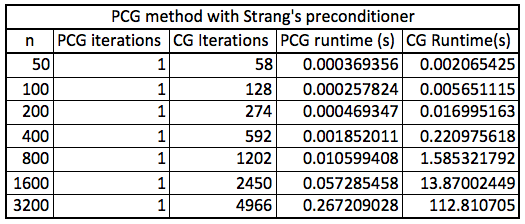
\includegraphics[width=120mm]{pcsb.png}
\caption{The final runtimes of the CG iterative method and the PCG iterative method with a Strang circulant preconditioner.}
\label{pcgB1}
\end{center}
\end{figure}
 As can be seen in Figures \ref{pcgB1} and \ref{pcgB2}, the PCG method greatly outpaces the CG method in both runtime and number of iterations required to converge. However, once again the Chan and Strang circulant preconditioners are roughly equivalent. Both methods are able to converge within one iteration and both methods are able to handle the large matrices without issue. A brief analysis of the runtimes show that the $\approx$ \bigo($n\,log\,n$) growth rate discussed above is maintained with the second symmetric Toeplitz system analyzed here. 
 
 
\begin{figure}[htbp]
\begin{center}
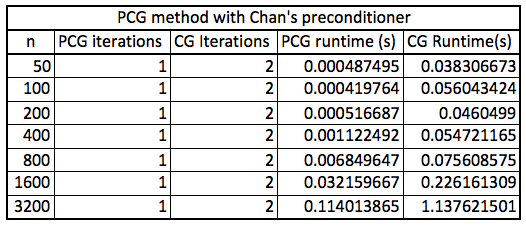
\includegraphics[width=120mm]{pccb.png}
\caption{The final runtimes of the CG iterative method and the PCG iterative method with a Chan circulant preconditioner.}
\label{pcgB2}
\end{center}
\end{figure}
 

%\begin{figure}[htbp]
%\begin{center}
%\begin{tabular}{ | l | c|c| c| c | c | c| c| c| c  | c | }
%\hline
%  &A & B & C &D &E&F&G&H&I&J\ \\\hline
%  Design1 &240 & 350 & 305 & 30 & 35& 400& 90& 0& 30& 300 \\\hline
%% Design2 &300 & 380 & 370 & 34 & 40& 400& 100& 50& 100& 100 \\\hline
%%  Design3 &300 & 600 & 580 & 40 & 50& 550& 100& 150& 200& 250 \\\hline
%
%\end{tabular}
%\caption{Design 1 Parameters}
%\end{center}
%\end{figure}
%
%The isometric view of this design can be seen in Figure \ref{d1i}. The large cylinder was plotted using multiple instances of the \mcode{surf} command on two cylinders. Figure \ref{d1y} and Figure \ref{d1z} show the printer design in the X-Y and X-Z plains, respectively.
%
%\begin{figure}[htbp]
%\begin{center}
%\includegraphics[width=160mm]{d1iso.png}
%\caption{An isometric view of Design 1}
%\label{d1i}
%\end{center}
%\end{figure}



\end{document}  